\documentclass[12pt]{article}
\setcounter{secnumdepth}{5}
\usepackage{geometry}                % See geometry.pdf to learn the layout options. There are lots.
\geometry{letterpaper}                   % ... or a4paper or a5paper or ...
\usepackage{graphicx}
\usepackage{amssymb}
\usepackage{amsthm}
\usepackage{epstopdf}
\usepackage[utf8]{inputenc}
\usepackage[usenames,dvipsnames]{color}
\usepackage[table]{xcolor}
\usepackage{hyperref}
\usepackage{german}
\DeclareGraphicsRule{.tif}{png}{.png}{`convert #1 `dirname #1`/`basename #1 .tif`.png}

\theoremstyle{definition}
\newtheorem{example}{Example}

\usepackage{array}
\newcolumntype{L}[1]{>{\raggedright\let\newline\\\arraybackslash\hspace{0pt}}m{#1}}
\newcolumntype{C}[1]{>{\centering\let\newline\\\arraybackslash\hspace{0pt}}m{#1}}
\newcolumntype{R}[1]{>{\raggedleft\let\newline\\\arraybackslash\hspace{0pt}}m{#1}}


\newcommand{\projektname}{Fitervari: Train Together}
\newcommand{\doctype}{Pflichtenheft}
\newcommand{\projektleiter}{F. Gewessler}
\newcommand{\projektmitglieder}{L.Gaisbauer, C. Knoll}
%\newcommand{\documentstatus}{Submitted}
%\newcommand{\documentstatus}{Released}
\newcommand{\version}{V. 1.0}

\begin{document}
\begin{titlepage}
\begin{flushright}

\includegraphics[scale=.5]{htlleondinglogo.png}\\
\end{flushright}

\vspace{10em}

\begin{flushright}

\end{flushright}
\begin{center}
{\LARGE \doctype} \\[3em]
\end{center}
\pagebreak


\begin{flushleft}
\begin{tabular}{|l|l|}
\hline
Projektname & \projektname \\ \hline
Projektleiter & \projektleiter \\ \hline
Projektmitglierder & \projektmitglieder \\ \hline
Version & \version \\ \hline
\end{tabular}
\end{flushleft}

\end{titlepage}

\tableofcontents
\pagebreak

\section{Ist-Zustand}
\begin{itemize}
    \item Es wurde ein Mockup erstellt, welches alle masken der Fitervari-App abbildet. Bei der erstellung des Mockup standen die einfache Benutzbarkeit und die User-Experience im Vordergrund. 
    \item Das Datenmodell, sowie das Backend der Applikation sind weitestgehend fertig.
    \item Die Implementation des Frontends (Der Fitervari-App) wurde begonnen, wobei die Anzeige der Neuiggkeiten bereits an dem Backend angebunden ist.   
\end{itemize}

\pagebreak

\section{Zielsetzung}

\subsection{Ziele}
\begin{itemize}
\item Der Benutzer kann unbegrenzt Workouts hinzufügen und diese durchführen.
\item Der Trainer kann kundenspezifische Workouts erstellen und dem jeweligen Kunden zuordenen.
\item Der Benutzer kann sein Fortschritt in den jeweiligen Workouts anhand von Diagrammen und Auflistungen seinen vortschritt beobachten.
\item Der Benutzer wird informiert, ob ein anderer Nutzer in seinem Fitnessstudio ein Workout teilen möchte und welche Übungen dieses Workout enthält.
\item Auf der Startseite der Applikation werden neuigkeiten angezeigt.
\item Möglichst leichte bedienung und User-Experience.
\end{itemize}
\subsection{Erweiterungen}
\begin{itemize}
\item Vorschläge für personalisierte Workouts.
\item Trainer-Benutzer kommunikation.
\end{itemize}

\subsection{Nicht-Ziele}
\begin{itemize}
\item Vorschläge und Erstellen von Ernährungsplänen.
\item Management der Fittnesstudio mitgliedschaft.
\end{itemize}

\subsection{Alleinstellungsmerkmal}
Die Funktion sein Workout mit anderen zu teilen und diese zum Workout einzuladen, 
ist in der Industrie einzigartig. Die Applikation wird über eine minimalistische und innovative UI verfügen, 
die alle wichtigen Features und Funktionen zum Tracken von eigens zusammengestellten Workouts bereitstellt.

\pagebreak

\section{Anforderungen}

\subsubsection{App}

Um eine gute Userexperience sicher zu stellen, muss die App sehr simpel strukturiert und einfach zu verwenden sein. Ebenso wichtig ist es, dass die App auf allen Platformen (Android, IOS, Web) verfügbar ist um die Menge an potentiellen Nutzern nicht einzuschränken.

\paragraph{Kommunikationsstruktur}
\begin{center}

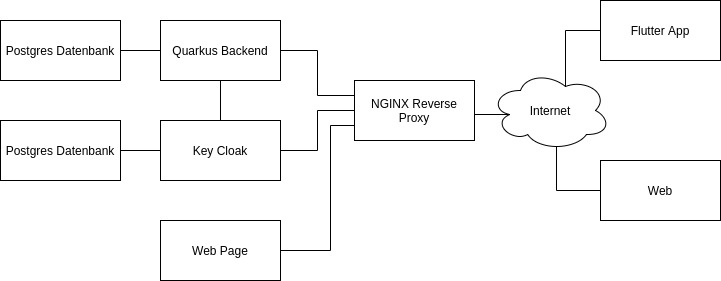
\includegraphics[width=15cm]{Kommunikationsdiagramm.jpg}

\end{center}
\pagebreak

\paragraph{Graphische Benutzeroberfläche}
\begin{flushleft}
Unsere Clientapplikation ist in Flutter geschrieben, was die Entwicklung erheblich beschleunigt. Desweiteren legen wir den Fokus auf einfache Bedienbarkeit und elegante, minimalistische Obtik.

\end{flushleft}

\begin{flushleft}

\end{flushleft}

\subsubsection{Server}
Der Server sollte 99\% der Zeit erreichbar sein um eine ununterbrochene Erfahrung zu bieten.\\
\paragraph{Datenmodel der Fitervari Datenbank}
\begin{center}

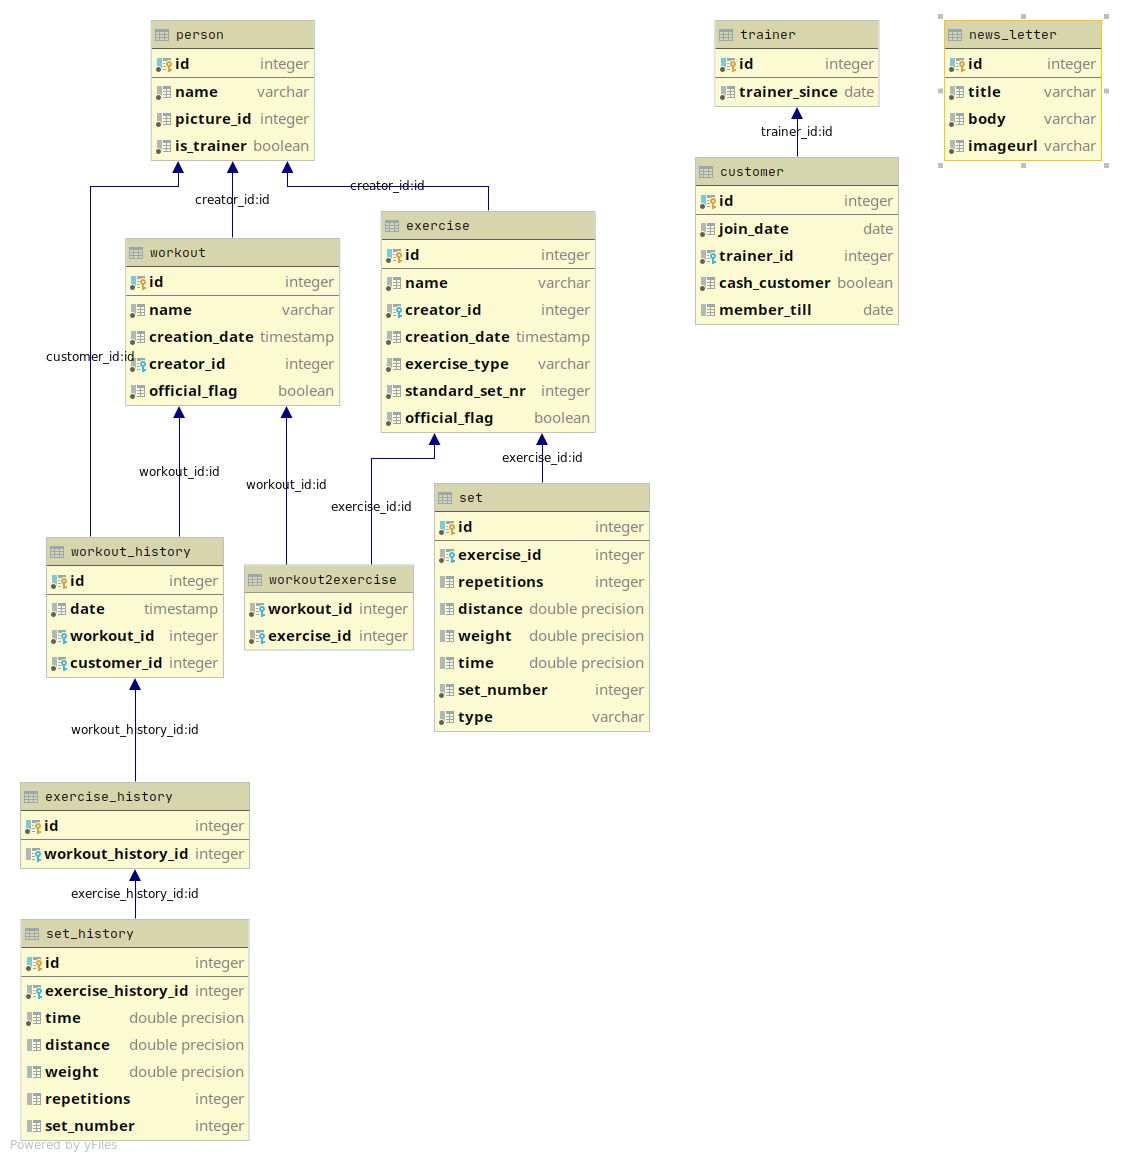
\includegraphics[width=15cm, height=12.6cm]{datenmodel.png}

\end{center}
\pagebreak

\subsubsection{Usecases}

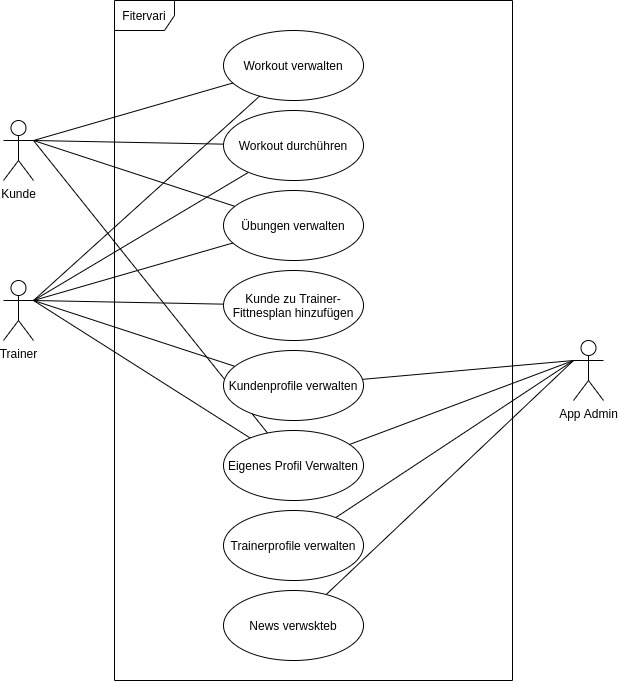
\includegraphics[width=15cm, height=18.5cm]{UseCase_Diagramm.jpg}

\newpage

\paragraph{App einrichten}
\begin{center}

\end{center}
\begin{center}
\begin{tabular}{| L{3cm} | C{12cm} |}
\hline
App installieren & Die Fitervari: Train Together-App wird sowohl im Google Play Store, als auch im App Store verfügbar sein. Um diese dann im jeweiligen Store zu finden, einfach in den Suchbereich „Fitervari“ eingeben, die App auswählen und diese dann wie gewohnt auf das Mobiltelefon installieren.\\

\hline
Registration & Zur Identifikation wird sich der User registrieren müssen. Der User wird sich also beim Starten der App einloggen müssen, damit die jeweiligen Daten geladen werden können.\\


\hline
\end{tabular}
\end{center}

\pagebreak
\subsubsection{Aktivitätsdiagramme}
\paragraph{Hardware über App verbinden}
\begin{center}

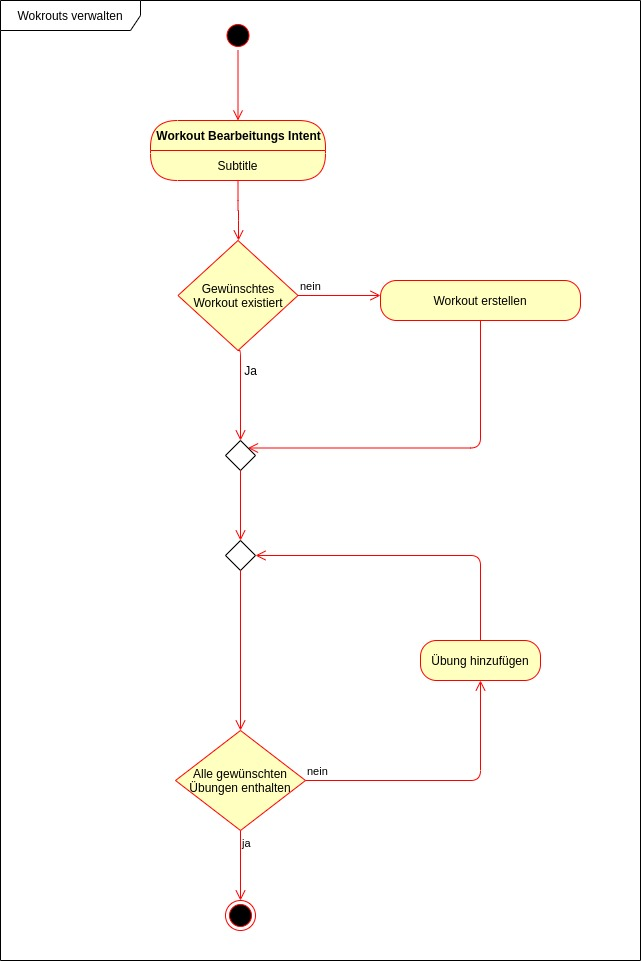
\includegraphics[width=11cm, height=17cm]{Aktivitaetsdiagramm.jpg}

\end{center}

\pagebreak
\section{Entwicklung}

\subsection{Frontend}

Die Frontend-Entwicklung ist mit dem Crossplatform-Framework Flutter, entwickelt von Google, umgesetzt.

\subsection{Backend}

Die Backend-Entwicklung ist in der Sprache Kotlin umgesetzt. Desweiteren wird hier das Quarkus-Framework verwendet.


\pagebreak

\section{Angebot}
\subsection{Angebot für Studioketten}

Der Plan ist, dass ein Fitnessstudio bei Fitervari unter Vertrag steht und eine gewisse Gebühr an Fitervari zahlt. Das Fitnessstudio selbst gibt die App an ihre Kunden kostenlos weiter.


Preis nach Vertragsverhandlung

\subsection{Angebot für Freelancer-Trainer}

Freelancer-Trainer die Fitervari mit voller Funktionalität nutzen wollen, müssen ein Premium-Abo abschließen und zahlen somit 1€.

\subsection{Angebot für Privatkunden}

Privatkunden erhalten die Grundfunktionalität (ohne Trainerfunktion) kostenlos

\end{document}
